\documentclass[../main.tex]{subfiles}

\begin{document}
    \section{Tujuan}
        \begin{enumerate}
            \item Melakukan simulasi pemodelan \textit{mass spring damper} menggunakan simechanics
            \item Melakukan simulasi pemodelan \textit{inverted pendulum} menggunakan simechanics
        \end{enumerate}
    \section{Dasar Teori}
        Sistem mekanik merupakan sebuah sistem yang bekerja dengan memanipulasi gaya dan perpindahan. Salah satu contoh dari penerapan sistem mekanik yang sederhana adalah pegas dan damper. Untuk mengendalikan sistem - sistem mekanik secara tepat, hal yang harus diketahui adalah karakteristik dari sistem tersebut. Salah cara untuk memahami karakteristik sistem adalah dengan melakukan identifikasi dan simulasi terhadap sistem tersebut untuk mengetahui performa dan karakteristik sistem\cite{Fahmizal}. salah satu perangkat lunak yang digunakan dalam simulasi kendali adalah MATLAB. MATLAB memiliki fitur untuk mendukung simulasi sistem mekanik menggunakan \textit{simechanics}.
    \section{Hasil dan Pembahasan}
        \subsection{Pemodelan Mass Spring Damper pada Simechanics}
            Diagram sistem \textit{mass spring damper} ditunjukkan pada gambar \ref{diagram_msd}.
            \begin{figure}[H]
                \centering
                \includegraphics[width = 0.5\textwidth]{assets/image/diagram_mass_spring_damper.png}
                \caption{Diagram Mass Spring Damper}
                \label{diagram_msd}
            \end{figure}
            \begin{center}
                Keterangan : 
                \begin{minipage}[c]{8cm}
                    \begin{itemize}
                        \item $k$ : konstanta pegas
                        \item $b$ : konstanta damper
                        \item $m$ : massa benda
                        \item $x_{(t)}$ : posisi
                        \item $f_{(t)}$ : gaya
                    \end{itemize}
                \end{minipage}
            \end{center}
            \subsubsection{Pemodelan sistem secara matematis}
                Pemodelan matematis dari sistem \textit{mass spring damper} dapat dilakukan dengan persamaan Newton yang ditunjukkan pada \eqref{persamaan_1}.
                \begin{equation}
                    \sum F = ma
                    \label{persamaan_1}
                \end{equation}
                Dari diagram sistem pada Gambar \ref{diagram_msd} dapat dianalisis gaya-gaya yang bekerja pada sistem. Analisis terhadap gaya sistem menghasilkan persamaan yang mendeskripsikan \textit{state} sistem berupa percepatan seperti yang ditunjukkan pada persamaan \eqref{persamaan_2}.
                \begin{equation}
                    \begin{split}
                        u - kx - b\dot{x} &= m\ddot{x}\\[5pt]
                        \frac{1}{m}u - \frac{k}{m}x - \frac{b}{m}\dot{x} &= \ddot{x} \\[5pt]
                        -\frac{b}{m}\dot{x} - \frac{k}{m}x + \frac{1}{m}u &= \ddot{x}
                        \label{persamaan_2}
                    \end{split}
                \end{equation}
                Dari persamaan \eqref{persamaan_2} diketahui sistem memiliki dua \textit{state} yaitu posisi ($x$) dan kecepatan ($\dot{x}$). untuk memudahkan proses analisis sistem. dibuat aturan penamaan \textit{state} sebagaimana ditunjukkan pada persamaan \eqref{persamaan_3}.
                \begin{equation}
                    \begin{split}
                        x_1 &= x\\[5pt]
                        x_2 &= \dot{x_1} = \dot{x}
                        \label{persamaan_3}
                    \end{split}
                \end{equation}
                Dari persamaan \eqref{persamaan_2} dan aturan pada persamaan \eqref{persamaan_3} maka model \textit{state space} dapat dicari. Hasil pemodelan \textit{state space} sistem ditunjukkan pada \eqref{persamaan_4}
                \begin{equation}
                    \begin{split}
                        \dot{x} &= Ax + Bu \\[5pt]
                        \begin{bmatrix} \dot{x_1} \\ \dot{x_2} \end{bmatrix} &= \begin{bmatrix} 0 & 1 \\ -\frac{k}{m} & -\frac{b}{m} \end{bmatrix} \begin{bmatrix} x_1 \\ x_2 \end{bmatrix} + \begin{bmatrix} 0 \\ \frac{1}{m} \end{bmatrix} u\\[10pt]
                        y &= Cx+Du \\[5pt]
                        y &= \begin{bmatrix} 1 & 0 \end{bmatrix} \begin{bmatrix} x_1 \\ x_2 \end{bmatrix}
                        \label{persamaan_4}
                    \end{split}
                \end{equation}
            \subsubsection{Validasi analisis matematis dengan MATLAB}
            Model matematis sistem pada persamaan \eqref{persamaan_4} diverifikasi untuk melihat respon sistem. untuk memperoleh respon sistem, sistem diberikan input \textit{step} dengan parameter sistem sebagaimana ditunjukkan pada Tabel \ref{parameter_msd}
                \begin{table}[H]
                    \centering
                    \caption{Parameter simulasi \textit{mass spring damper}}
                    \label{parameter_msd}
                    \begin{tabular}{|c|l|r|}
                        \hline
                        Reference & \multicolumn{1}{c|}{Parameter} & \multicolumn{1}{c|}{Value} \\ \hline
                        k         & spring constant                & $150N/m$                   \\ \hline
                        b         & damping constant               & $1 N/(m/s)$                \\ \hline
                        m         & mass                           & $1kg$                      \\ \hline
                        u         & input force                    & $10N$                      \\ \hline
                    \end{tabular}
                \end{table}
                Program simulasi dilakukan untuk mendapatkan gambaran umum mengenai karakteristik sistem. program untuk simulasi sebagai berikut,
                \lstinputlisting[language = matlab]{assets/code/validasi_msd.m}
                Hasil \textit{console} program menunjukkan model matematis yang sesuai dengan Persamaan \eqref{persamaan_4}. Keluaran \textit{console} sebagai berikut,
                \lstinputlisting[language = matlab]{assets/code/console_validasi_msd.m}
                Grafik respon sistem ditunjukkan pada Gambar \ref{respon_step_msd}. Respon sistem merupakan posisi \textit{mass spring damper}, dari data yang diamati, sistem memiliki osilasi. Namun, osilasi terlihat menurun seiring bertambahnya waktu. Dapat disimpulkan, sistem memiliki dan dapat menunuju kesetabilan.
                \begin{figure}[H]
                    \centering
                    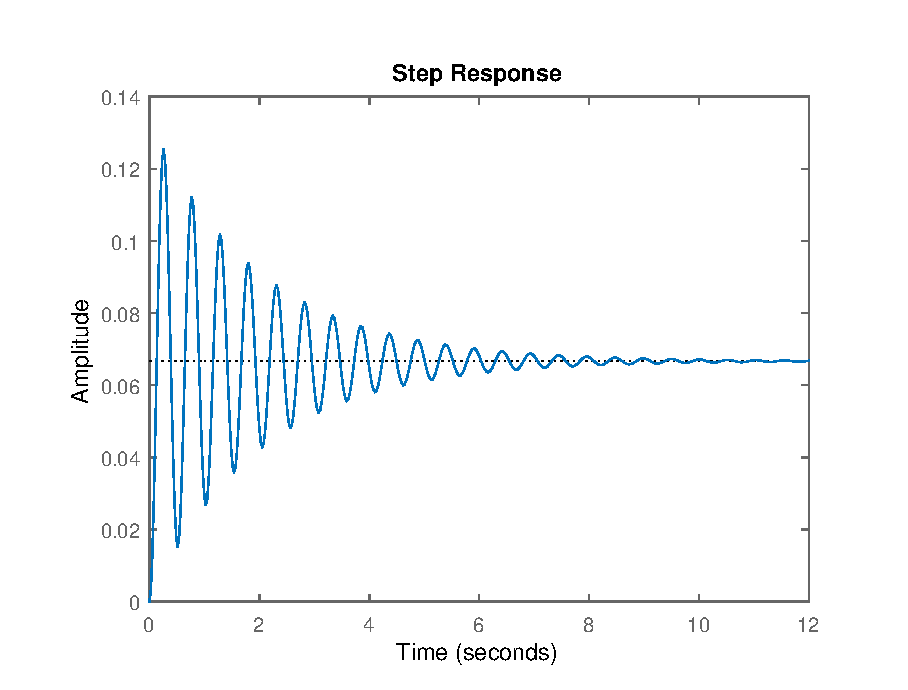
\includegraphics[width =0.8\textwidth]{assets/image/validasi.eps}
                    \caption{Respon sistem dengan input step}
                    \label{respon_step_msd}
                \end{figure}
            \subsubsection{Simulasi Mass Spring Damper pada Simechanics}
                Simulasi dilakukan pada \textit{simscape} dan \textit{simechanics} untuk memahami respon sistem dengan lebih baik dikarenakan pada \textit{simechanics} dapat menampilkan representasi 3D dari sistem yang diujikan. Diagram untuk simulasi pada \textit{simscape} dan \textit{simechanics} ditunjukkan masing-masing pada Gambar \ref{simulasi_simulink} dan Gambar \ref{simulasi_simscape}.
                \begin{figure}[H]
                    \centering
                    \includegraphics[width = 0.6\textwidth]{assets/image/mass_spring_damper_simulink.pdf}
                    \caption{Diagram blok simulasi sistem menggunakan simulink}
                    \label{simulasi_simulink}
                \end{figure}
                \begin{figure}[H]
                    \centering
                    \includegraphics[width = 0.6\textwidth]{assets/image/mass_spring_damper_simscape.pdf}
                    \caption{Diagram blok simulasi sistem menggunakan simscape}
                    \label{simulasi_simscape}
                \end{figure}
                Hasil dari simulasi menggunakan \textit{simscape} dan \textit{simechanics} deibandingkan sebagaimana ditunjukkan pada Gambar \ref{hasil_simulasi_simulink_simscape}. Dari hasil tersebut diamati bahwa data hasil simulasi \textit{simscape} dan \textit{simechanics} berhimpit. Hal ini terjadi karena data dari kedua simulasi memiliki selisih yang sangat kecil. Dari data ini dapat dilihat bahwa pemodelan sistem memiliki hasil yang konsisten menggunakan \textit{simscape} dan \textit{simechanics}.
                \begin{figure}[H]
                    \begin{tikzpicture}[trim left = -1cm]
                        \begin{axis}
                            [   width = \textwidth,
                                height = 0.5\textwidth,
                                xlabel={time}, 
                                ylabel={system respond}, 
                                grid, 
                                xmin=0, 
                                xmax=10, 
                                ymin=0, 
                                ymax=0.13, 
                                x label style={at{(axis description cs:0.5,-0.1)}},
                                axis lines = box,
                                tick align=inside,
                            ]
                            \addplot[red, no marks, smooth] table[col sep=space]{assets/data/mass_spring_damper_simulink.csv};
                            \addlegendentry{simulink}
                            \addplot[blue, no marks, smooth] table[col sep=space]{assets/data/mass_spring_damper_simechanics.csv};
                            \addlegendentry{simechanics}
                        \end{axis}
                    \end{tikzpicture}
                    \caption{Hasil simulasi sistem menggunakan simulink dan simscape}
                    \label{hasil_simulasi_simulink_simscape}
                \end{figure}
                Dari \textit{simechanics} juga dapat dilihat model 3D dari sistem \textit{mass spring damper} sebagaimana ditunjukkan pada Gambar \ref{simulasi_3d_msd}. Dari hasil tersebut model diamati bergerak translasi pada satu sumbu, sistem bergerak maju mundur. Pergerakan maju mundur ini berkurang seiring bertambahnya waktu. Gerak sistem ini sesuai dengan grafik respon sistem pada Gambar \ref{hasil_simulasi_simulink_simscape}.
                \begin{figure}[H]
                    \centering
                    \includegraphics[width = 0.6\textwidth]{assets/image/MecahnicExplorer.png}
                    \caption{Hasil tampilan simulasi 3D model dari sistem \textit{mass spring damper}}
                    \label{simulasi_3d_msd}
                \end{figure}
        \subsection{Pemodelan Inverted Pendulum pada Simechanics}
            Pemodelan pada inverted pendulum tidak dapat dilakukan karena add-ins \textit{simulink multibody} tidak dapat ditampilkan pada \textit{menubar tools} walaupun \textit{add-ins sudah diaktifkan}. Sehingga, tidak dapat dilakukan konversi dari model 3D ke model \textit{simechanics}.
            \begin{figure}[H]
                \centering
                \includegraphics[width = 0.6\textwidth]{assets/image/error_add_ins.png}
                \caption{\textit{Add-ins} \textit{simulink multibody} telah terpasang pada MATLAB dan muncul pada pilihan \textit{add-ins} pada solidWorks}
                \label{error_add_ins}
            \end{figure}
            \begin{figure}[H]
                \centering
                \includegraphics[width = 0.6\textwidth]{assets/image/error_menubar_tools.png}
                \caption{Pilihan menu \textit{simulink multibody} pada \textit{tools} tidak ada walaupun pada opsi \textit{add-ins} sudah diaktifkan}
                \label{error_menu}
            \end{figure}
    \section{Kesimpulan}
        Dari hasil dan pembahasan diatas, dapat ditarik kesimpulan sebagai berikut,
        \begin{enumerate}
            \item Simulasi pemodelan sistem \textit{mass spring damper} pada MATLAB dapat dilakukan dengan \textit{simscape} dan \textit{simechanics} untuk mendapat gambaran mengenai karakteristik sistem melalui grafik respon sistem dan pemodelan 3D dari sistem \textit{mass spring damper}
            \item Simulasi \textit{inverted pendulum} belum dapat dilakukan karena terdapat error pada \textit{add-ins} s\textit{simulink multibody} yang menyebabkan model 3D dari solidWorks tidak dapat dikonversi menjadi model mekanik di MATLAB. 
        \end{enumerate}
    \begin{thebibliography}{2}
        \bibitem[1]{Fahmizal} Fahmizal. 2020. "Pemodelan dan Identifikasi Sistem" dalam \textit{Modul Praktikum Teknik Kendali Lanjut} (hlm.1-8). Yogyakarta
    \end{thebibliography}
\end{document}